\chapter{The CMS Experiment}

In the previous chapter we summarized the theoretical underpinnings of modern
particle physics, and discussed possible extensions that point towards
future research. We now turn our attention to the machines that make such
research possible. The Large Hadron Collider (LHC) is the largest
particle collider ever built, smashing protons together at record energies.
On it are located four major experiments, designed to record electrical
snapshots of the collisions and allow physicists to reconstruct the details
of each event. Sec.~\ref{sec:lhc} describes the design and operation of the LHC,
and Sec.~\ref{sec:cms_det} introduces the Compact Muon Solenoid (CMS) experiment,
one of the four at the LHC and the one used for the analysis in this dissertation.

\section{The Large Hadron Collider}
\label{sec:lhc}

Underneath the French-Swiss border near the city of Geneva lies the LHC, the world's largest 
proton collider. With a circumference of 26.7 kilometers and depth of up to 175
meters below ground, it is designed to accelerate protons to an energy of 7\TeV, over
7,000 times their rest mass (and corresponding to a speed 
99.9999991\% the speed of light). Utilizing the tunnel of the older Large Electron--Positron
collider (LEP) at CERN, it was constructed to supersede the Tevatron at Fermilab, which
accelerated protons to 1\TeV.

What was the motivation for such a machine? The LEP collider, which accelerated electrons
and positrons to up to 209\GeV, had allowed for precise measurements of many SM quantities
inclusing the $W$ and $Z$ masses, but was not able to find definitive proof of a Higgs boson
or any evidence for BSM physics. Similarly, the Tevatron had discovered the top quark
and made many measurements but failed to find evidence of the Higgs or new physics. Physicists
thus sought a next-generation machine that could find these things.

\begin{figure}[t]
  \begin{center}
    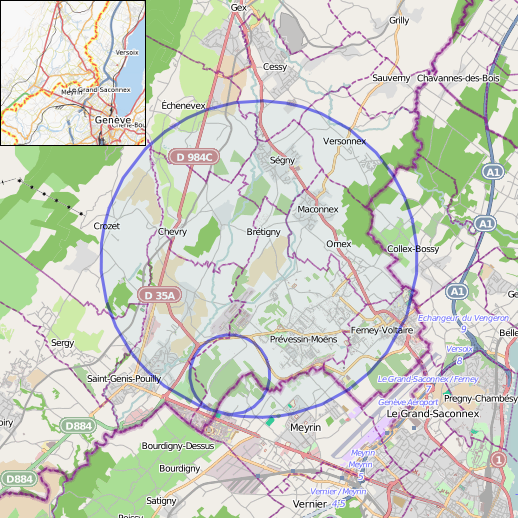
\includegraphics[width=0.39\textwidth]{figs/cms/lhc_osm.png}
    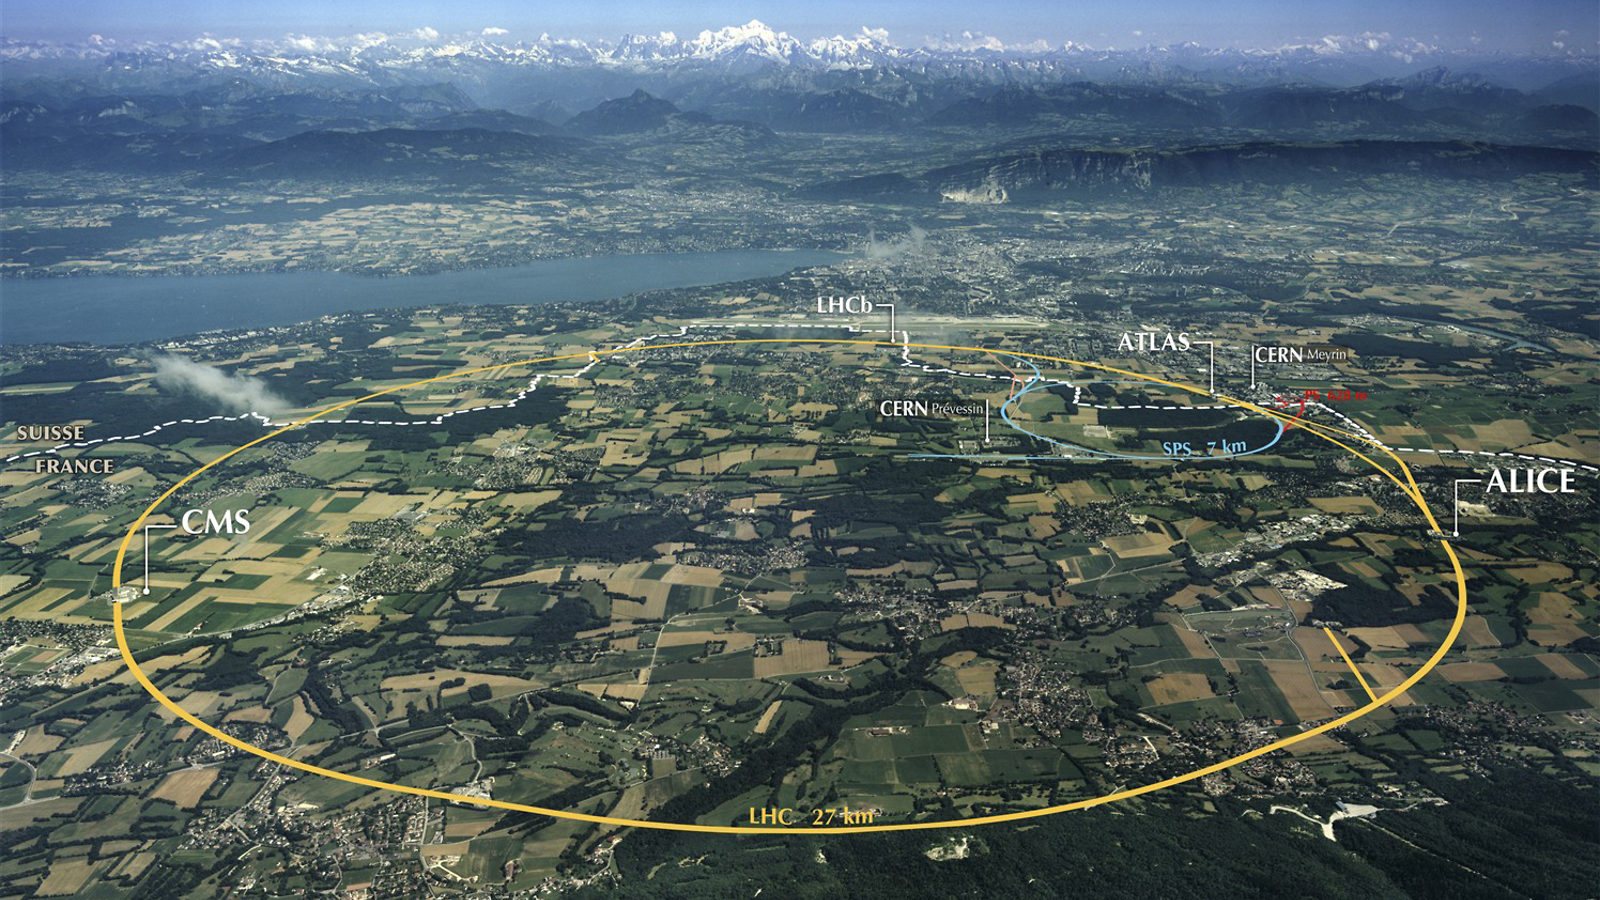
\includegraphics[width=0.59\textwidth]{figs/cms/lhc_photo.jpg} 
    \caption{(left) The SPS and LHC overlaid on a map of the Franco-Swiss border near Geneva. The diameter of
      the LHC is 8.5 km (5.3 miles). (right) The LHC, the four major experiments, and CERN's campus 
      overlaid on a photo of the Geneva area, looking southeast. Lake Geneva and the French Alps can
      be seen in the background. (Images from \cite{lhc_map,lhc_photo})
            }
    \label{fig:lhc}
  \end{center}
\end{figure}

Since the Higgs and potential new physics were at energy scales above the reach of
present experiments, a higher energy collider was needed. 
Circular lepton colliders like LEP
are limited in energy, as the energy radiated by an accelerating charged particle falls as 
$1/m^4r^2$, and so the size of the necessary electron collider would be prohibitive.
The much heavier proton is far easier to accelerate to high energies, and an accelerator
in the pre-existing LEP tunnel was sufficient to achieve the necessary energies
(and additionally, cost-effective).
The downside is that collisions of composite particles like protons are messy, and
the actual parton collision energy is indeterminate. However, the LHC was meant do be a 
``discovery machine'', so probing a wide range of collision energies was desirable.
For precision studies of any interesting physics uncovered by the LHC, a future
linear $e^+e^-$ collider would be a good option.

From these considerations, the particle physics community 
decided on a $pp$ collider built in the LEP tunnel,
and construction on the LHC began in 1998. A map of its location can be seen in
Fig.~\ref{fig:lhc}. It sits in a tunnel between 50 and 175 meters underneath
the suburbs of Geneva, Switzerland, straddling the France-Switzerland border.
To the west are the Jura mountains, and to the east Lake Geneva. The CERN
campus is on the south end.

\begin{figure}[t]
  \begin{center}
    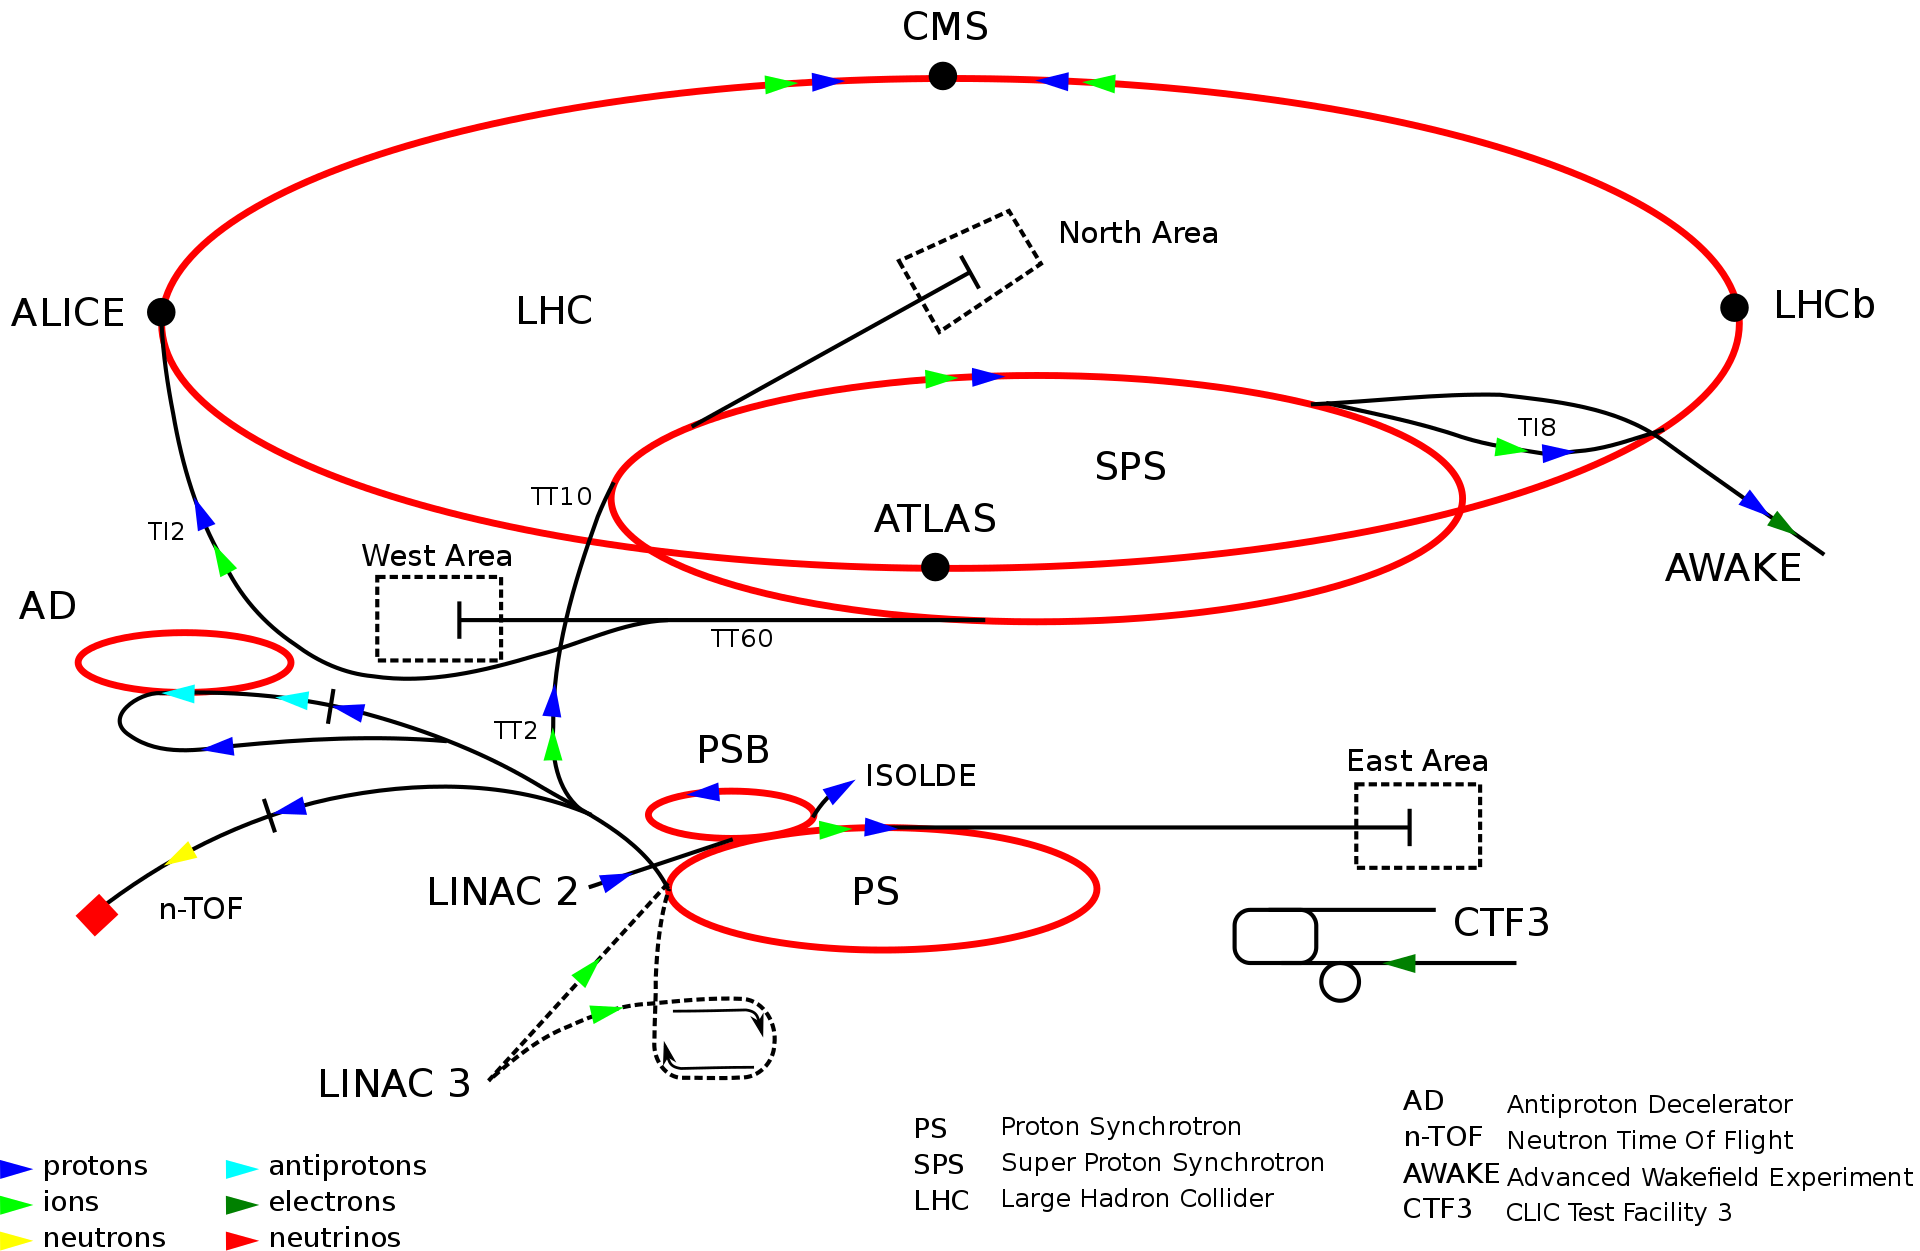
\includegraphics[width=0.60\textwidth]{figs/cms/accelerator_complex.png}
    \caption{The CERN accelerator complex. Protons originate in the LINAC 2 where they are 
      injected at 50\MeV into the PSB. The PSB, PS, and SPS subsequently accelerate them
      to 1.4\GeV, 26\GeV, and 450\GeV, respectively, before they enter the LHC where they
      reach up to 6.5\TeV. (Image from~\cite{accelerator_complex})
            }
    \label{fig:cern_accelerator_complex}
  \end{center}
\end{figure}

Before entering the main ring, the protons progress through a series of
increasingly large accelerators. The steps in the chain are as follows;
the CERN accelerator complex is
illustrated in Fig.~\ref{fig:cern_accelerator_complex}. 
\begin{itemize}\setlength\itemsep{-1mm}
\item The protons begin as nuclei in hydrogren gas, and electric fields are used to strip the electrons away.
\item The bare protons are fed into the linear LINAC 2 accelerator, where
they are boosted to 50\MeV kinetic energy and injected into the 160 meter
Proton Synchrotron Booster (PSB).
\item The PSB accelerates the protons to 1.4\GeV and feeds them into the
628 meter Proton Synchrotron (PS).
\item The PS accelerates them to 26\GeV and injects them into the
6.9 kilometer Super Proton Synchrotron (SPS).
\item The SPS accelerates them to 450\GeV before finally injecting
them into the main 26.7 kilometer LHC ring (it inserts two beams, traveling
in opposite directions)
\item Over a period of around 20 minutes, the LHC accelerates the protons
to 6.5\TeV (this is the present maximum; the LHC is designed to eventually
go to 7\TeV).
\end{itemize}

In order to steer the beams in a circle, the LHC makes use of powerful superconducting
magnets. Dipole magnets are used as the main steering mechanism. From the formula 
for a relativistic charged particle in a uniform magnetic field, the necessary average
magnetic field is $B=\gamma m\beta/qR=5.1~\mrm{T}$. However, the magnets are not all the
way around the ring so the peak dipole magnetic field is 7.74 T. In addition to the dipole magnets,
quadrupole magnets are used for beam focusing, and higher multipole magnets are used for finer
corrections. In total there are nearly 10,000 individual magnets. In order to maintain a such a
strong field, the superconducting magnets operate at a temperature of only 1.9 K, achieved
using 96 tons of superfluid helium~\cite{lhc_guide}.

Magnets can only steer the beam, not increase its energy. In order to perform
the acceleration from 450\GeV to 6.5\TeV, the LHC makes use of 8 radio-frequency
(RF) cavities per direction that produce an oscillating electric field at a frequency of
400 MHz. This naturally produces a beam of ``bunches'', spaced 25 ns apart:
the electric fields boost the protons, and the gradient of the field is
constructed in such a way that any protons that arrive early or late
recieve a slightly different kick, pushing them back towards the bunch
center.

Together, the magnetic and electric fields produce two counter-rotating
beams of 6.5\TeV protons, organized into bunches 25 ns apart (corresponding
to around 7.5 m of spatial separation). There are about
$1.2\times10^{11}$ protons per bunch, and up to 2808 bunches per beam, giving
$3.4\times10^{14}$ protons in each beam. At 6.5\TeV each, the total kinetic energy
in both beams together is over 700 million joules, equivalent
to a Boeing 737 traveling at 200 mph!

The ``collision rate'' at colliders is measured with a quantity known as instantaneous
luminosity, defined by the rate $N$ of a given type of interaction with cross section (roughly, likelihood
of interaction) $\sigma$ as $\mathcal{L}=N\sigma$. This luminosity is a function of
the bunch crossing rate (at the LHC, once every 25 ns), the number of protons
per bunch, and the effective area of the beam (i.e., how tightly packed
the protons in the beam are). The LHC can reach an instantaneous luminosity of
around $2\times10^{34}~\mrm{cm}^{-2}\mrm{s}^{-1}$.

The total proton-proton inelastic cross section is measured to be around 78 mb~\cite{ATLAS:ppxsec}.
Multiplying by the LHC instantaneous luminosity, that means we expect
1.5 billion inelastic collisions per second, or around 40 per bunch crossing.
Most of these will be relatively uninteresting, and a major challenge in analyzing experimental
data is disentagling the interesting event from the $\sim40$ other interactions
(referred to as \textit{pileup} interactions).

The LHC began beam operations in September 2008. Just nine days after the
first beams circulated, an electrical fault led to the loss of
six tons of liquid helium, causing a magnet quench and an explosion
that damaged 53 magnets~\cite{LHC_incident}. This delayed the start of physics by a year until
November 2009, and limited the collision energy in the LHC's first run to 8\TeV.
This Run 1 lasted through the beginning of 2013, before a two year shutdown
and the start of 13\TeV collisions in Run 2 in 2015.

The LHC steers the counter-rotating beams to collide at four pre-defined
experimental interaction points, corresponding to the ATLAS, ALICE,
CMS, and LHCb experiments (illustrated in Figs.~\ref{fig:lhc} (right)
and \ref{fig:cern_accelerator_complex}).
ALICE is optimized to study collisions of Pb nuclei
(another capability of the LHC, and the reason for the use of 
``hadron collider'' instead of ``proton collider''), which
produce quark--gluon plasma. LHCb is an asymmetric forward
detector meant to study processes involving $B$ hadrons.
CMS and ATLAS are both general-purpose hermetic detectors,
meant to study a wide range of physics. 
We now turn our attention to the CMS experiment, which was used
to collect the data utilized in the present analysis.


\section{The CMS detector}
\label{sec:cms_det}

The Compact Muon Solenoid (CMS) detector is one of two general-purpose detectors
at the LHC, designed to capture the details of proton-proton collisions
as completely as possible in order to study the SM and search for any signs
of physics beyond the SM.

CMS is 21 meters long and 15 meters in diameter (relatively ``compact'', compared
to ATLAS). It is built around a central solenoidal magnet, which
provides a powerful magnetic field that bends the trajectories of charged
particles. The detector consists of various layers of sub-detectors and components,
illustrated in the cutaway diagram in Fig.~\ref{fig:cms_diagram}. The layers,
working from the inside out, are: the beampipe; silicon tracker;
electromagnetic calorimeter; hadronic calorimeter; magnet; muon detectors;
and steel return yokes (these last two are interspersed in alternating layers).
Moreover, these components are organized into a central cylindrical barrel,
providing coverage out to roughly 25$^\circ$ from the beamline,
and two circular endcaps that can be pulled away for access to the detector.
Photos of an opened CMS (i.e. with the endcaps pulled away) are shown in 
Fig.~\ref{fig:cms_photos}.

\begin{figure}[t]
  \begin{center}
    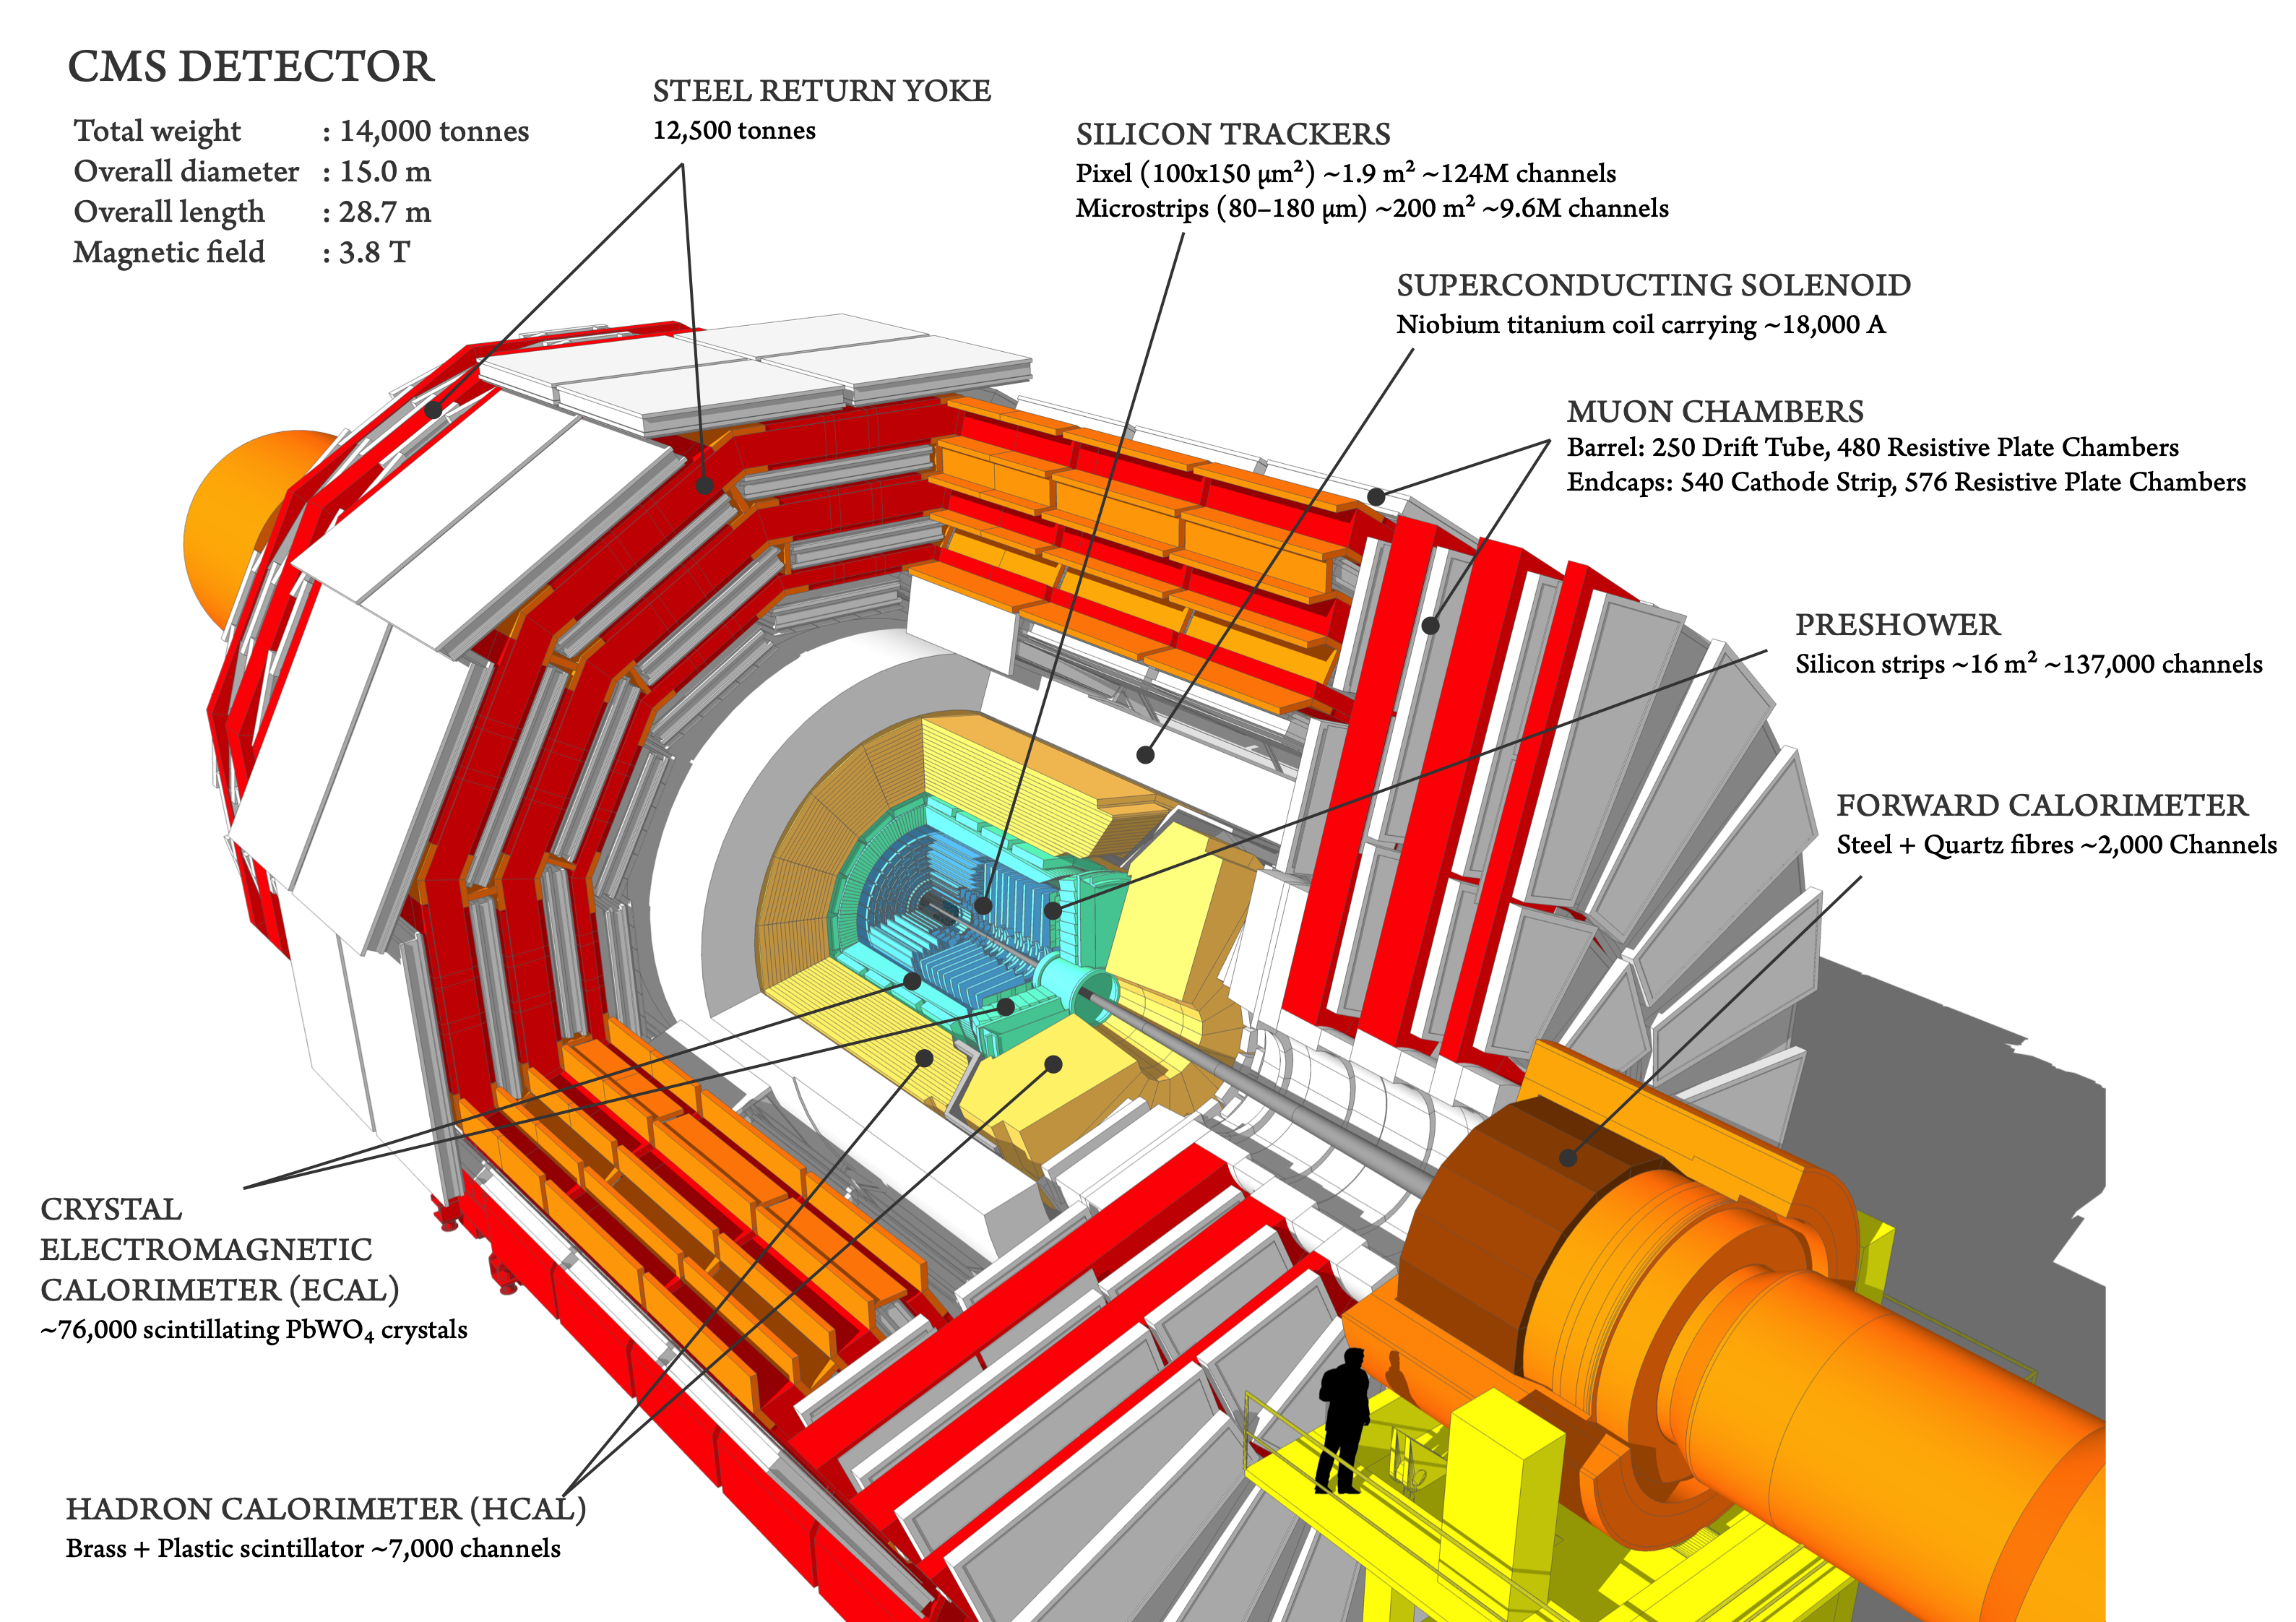
\includegraphics[width=0.99\textwidth]{figs/cms/cms_diagram.png}
    \caption{Cutaway illustration of the CMS detector. Note the outline
      of a human in the lower right for scale. (Image from~\cite{cms_vis})
            }
    \label{fig:cms_diagram}
  \end{center}
\end{figure}

\begin{figure}[t]
  \begin{center}
    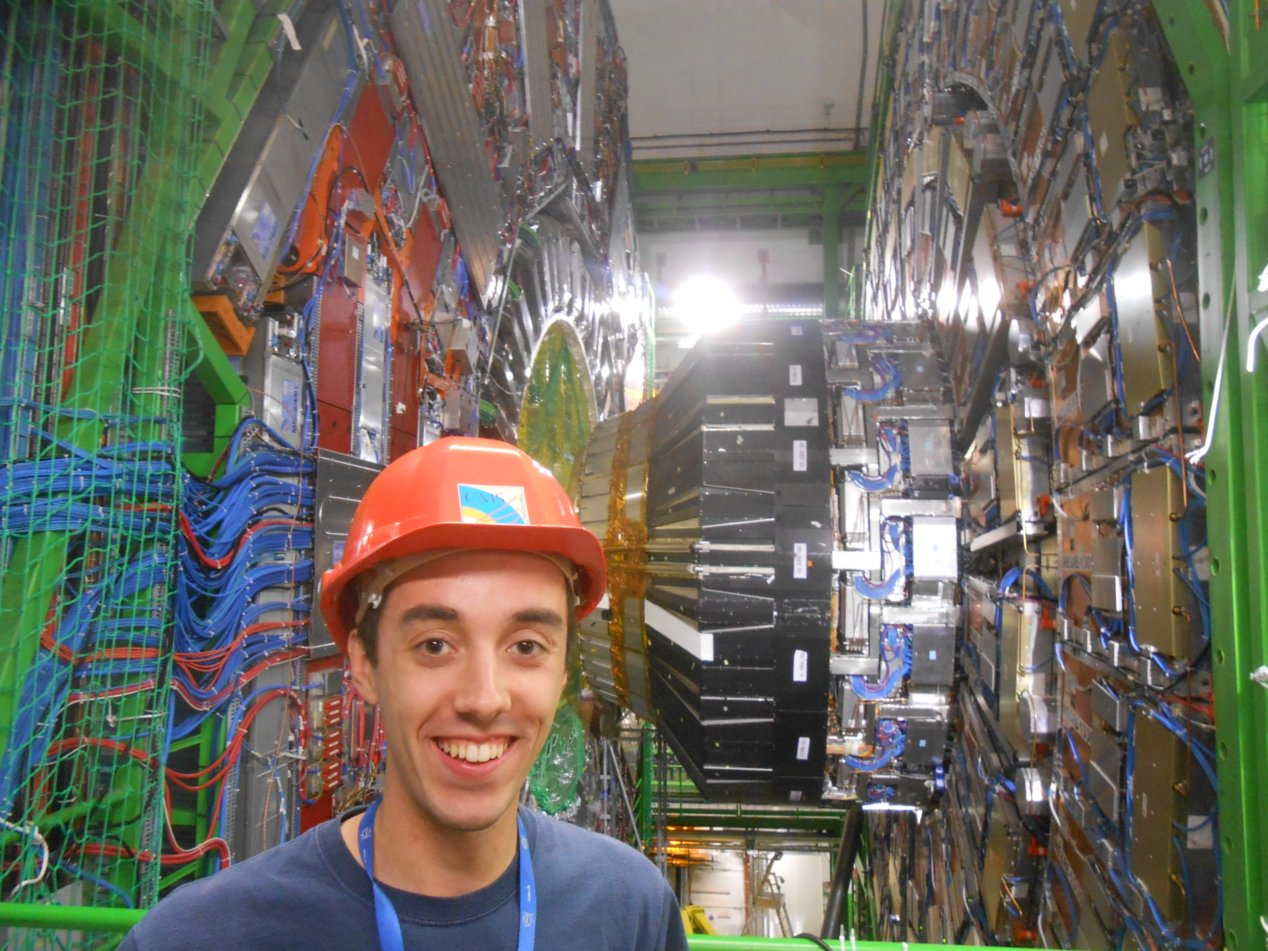
\includegraphics[width=0.45\textwidth]{figs/cms/bennett.jpg}
    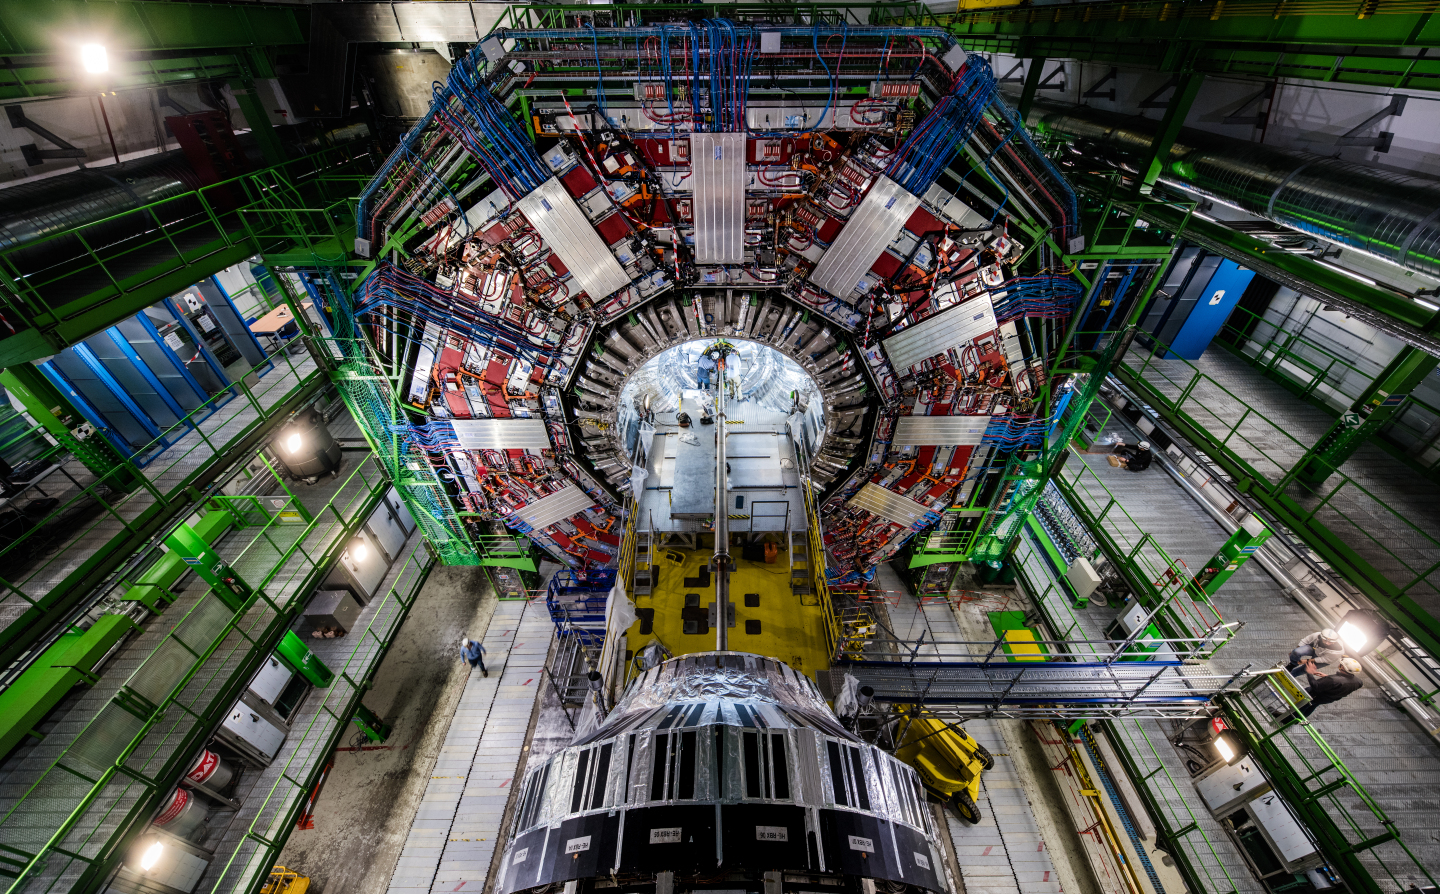
\includegraphics[width=0.54\textwidth]{figs/cms/cms_photo.jpg}
    \caption{(left) The author next to an opened CMS detector in summer 2014.
      On the right side is the muon endcap detector, with the endcap hadronic calorimeter
      protruding. On the left is the barrel, with the muon detectors and iron yokes
      on the outside, and the magnet forming the inner ring.
      (right) A broader view of the opened CMS detector, during the installation
      of the new phase-1 upgrade pixel detector in 2017. Note the technicians
      inside the barrel for scale. (Image via Maximilien Brice, CERN)
            }
    \label{fig:cms_photos}
  \end{center}
\end{figure}

We now go through each of the components and briefly describe their design and operation.
More detailed accounts and the full technical details can be found in the CMS Technical
Design Reports (volume I contains detector performace and software~\cite{CMS:tdr_i}, and
volume II describes physics performance~\cite{CMS:tdr_ii}. There are also more recent reports
describing various detector upgrades).

First, a word on coordinates and notation (used in this chapter and throughout this
dissertation): the standard CMS coordinate system is centered on the nominal collision
point, with the $x$ axis pointing radially inward toward the center of the LHC, the
$y$ axis pointing vertically upward, and the $z$ axis pointing along the beamline,
counter-clockwise if looking at the LHC from above. The coordinate $r$ refers to the 
cylindrical radius $r=\sqrt{x^2+y^2}$, and $\phi$ the azimuthal angle $\tan(\phi)=y/x$.
Instead of the polar angle $\theta=\tan^{-1}(r/z)$, particle physicists generally use
psudorapidity $\eta=-\log(\tan(\theta/2))$. The reason is that for relativistic
particles, $\eta$ is a very good approximation of rapidity, and differences in
rapidity are invariant under Lorentz boosts along the $z$ axis. A pseudorapity
of 0 is central (i.e. orthogonal to the beamline), and a pseudorapidity high
in absolute value indicates something nearly parallel to the beamline.
A subscript T on a quantity (e.g. \pt)
indicates the transverse (i.e. $xy$) component.

\subsection{Magnet and return yoke}

The core of CMS is a large solenoid designed to produce a strong magnetic field. Charged
particle trajectories are curved by this field, allowing reconsruction of their momenta
(the radius of curvature is given by $R=\pt/qB$).
The solenoid is 13 meters long and has an inner radius of around 3 meters, making
it the largest solenoidal magnet ever built. The coils are made of superconducting
niobium-titanium, and carry a current of 18,160 A to produce a magnetic field of 3.8 T.

Outside of the magnet coils are three layers of steel (called the ``return yoke''),
which provide support and guide 
the exterior return field (to limit the field strength outside of the physical
detector). A map of the magnetic field magnitude in a cross-sectional
plane of CMS is shown in Fig.~\ref{fig:cms_bfield}. The central 13 m $\times$ 6 m
core is visible, along with the layers of steel return yoke that carry most of the
exterior field. Outside of these structures, the field is relatively small.

\begin{figure}[t]
  \begin{center}
    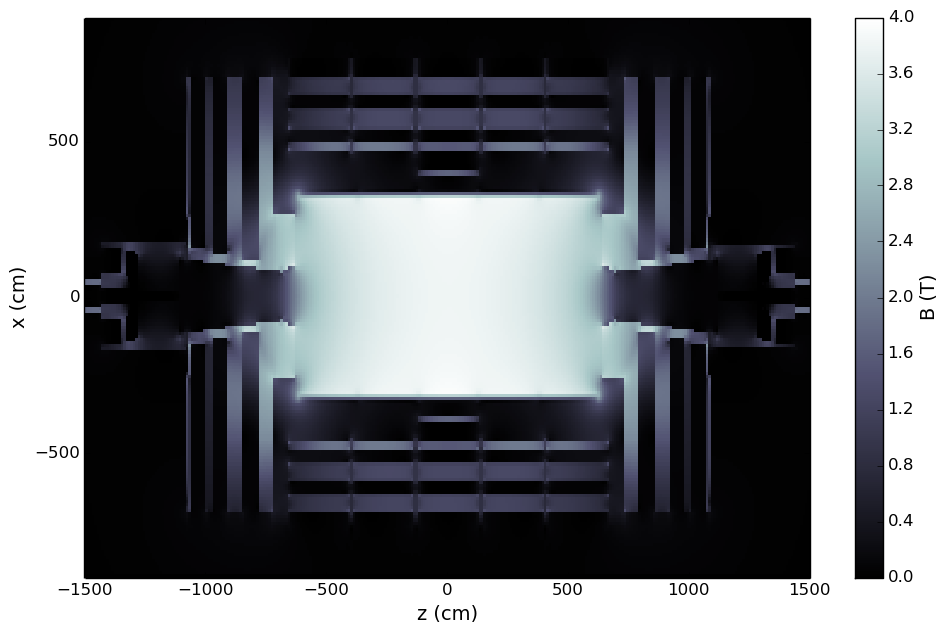
\includegraphics[width=0.60\textwidth]{figs/cms/cms_bfield_coarse.png}
    \caption{Map of the CMS magnetic field magnitude in an $rz$ cross-sectional plane.
      The magnitude is a roughly constant 3.8 T in the core inside the magnet coils, and weaker outside.
      The steel return yokes that carry back most of the magnetic flux are visible.
            }
    \label{fig:cms_bfield}
  \end{center}
\end{figure}

\subsection{Tracker}

The innermost detector, just outside of the beampipe and inside of the calorimeters and magnet,
is the silicon tracking detector. The aim of this detector is to accurately reconstruct the curved
trajectories of charged particles in order to reconstruct their momenta. 

A central challenge in the design of this detector is the radiation level so close to the beam: 
at 10 cm from the beampipe, the incident particle flux is around 10 million per cm$^2$ per second.
Hence, the detector must be radiation-hard. Additionally, material budget should remain
low so as to minimally affect the trajectories of through-going particles, and the detector
should give high spatial resolution and have fast response time, to allow accurate and timely
reconstruction of particle tracks.

From these considerations, a silicon detector was chosen, as silicon is relatively resilient
to radiation and has a fast response time. The detector works by reverse-biasing narrow
strips of silicon; throughgoing charged particles then ionize the atoms to create
electron-hole pairs, which can be collected via an voltage gradient and detected
as a small electrical pulse lasting a few nanoseconds.

%% \begin{figure}[t]
%%   \begin{center}
%%     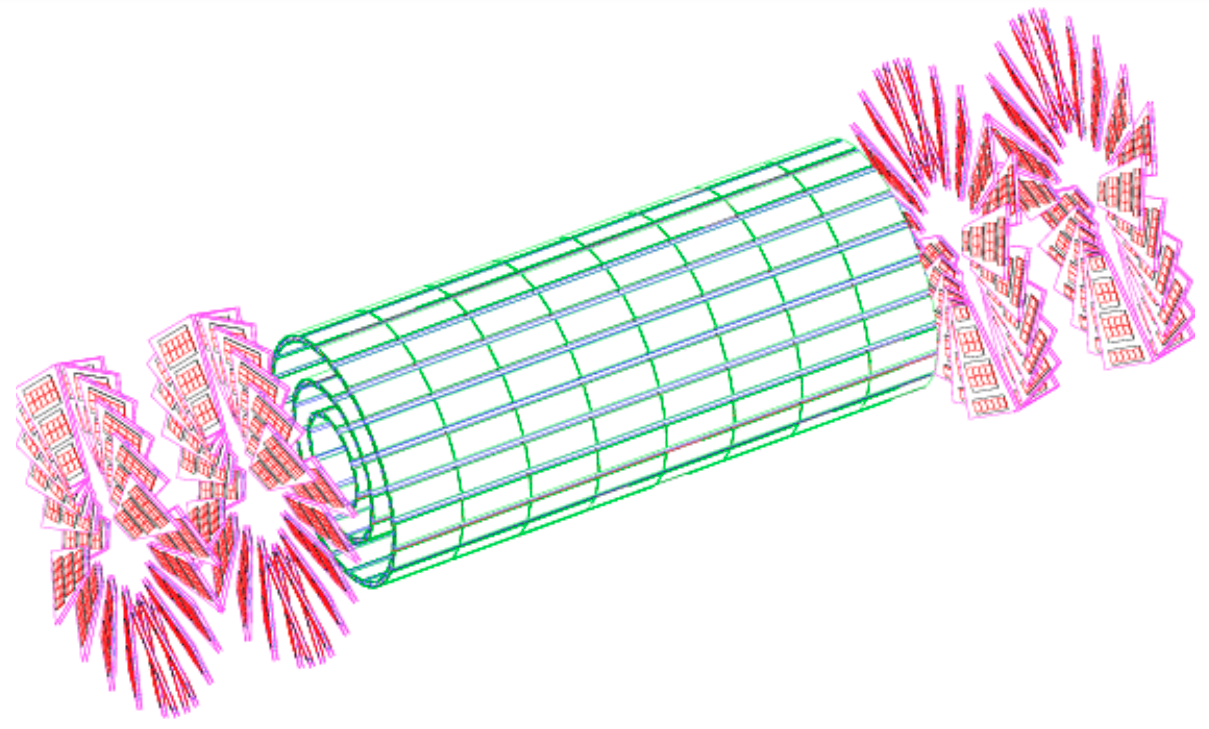
\includegraphics[width=0.50\textwidth]{figs/cms/tracker.png}
%%     \caption{Illustration of the pixel tracking layers. Note that this is the original layout;
%%       after the phase-1 upgrade in 2017, there is an additional layer in both the barrel
%%       and endcap systems. The pixel detector is 16 cm in radius and 100 cm long. (Image from~\cite{CMS:tdr_i})
%%             }
%%     \label{fig:cms_tracker}
%%   \end{center}
%% \end{figure}

The tracker consists of two main sub-modules. The first, called the pixel detector, 
is close to the beamline and consists of arrays of 100 $\mu$m $\times$ 150 $\mu$m
silicon pixels, with 124 million pixels in total.
There are four barrel layers at radii 2.9, 6.8, 10.9, and 16.0 cm,
and three endcap layers. The detector provides coverage out to $|\eta|<2.4$.
The small size of the pixels allows for highly accurate identification of particle location.
%% An illustration of the pixel detector layout (before the 2017 phase-1 upgrade, which added
%% additional layers to the barrel and endcap) is shown in Fig.~\ref{fig:cms_tracker}.

Outside of the pixel detector are 10 layers of silicon strips in the barrel, and 12 in the
endcaps. The four inner barrel layers
consist of 10 cm $\times$ 180 $\mu$m strips, and the next six consist of 
25 cm $\times$ 180 $\mu$m strips. There are 10 millions strips in total,
and the strip tracker reaches out to a radius of 130 cm.

\subsection{Electromagnetic calorimeter}

Between the tracker and the magnet lie two calorimeters. The first,
called the electromagnetic calorimeter (ECAL), is designed to
measure the energy of electrons and photons. It works by triggering
an electromagnetic shower: in the presence of matter, 
a high-energy electron will lose energy by emitting a photon
in a process called bremsstrahlung, and a high-energy photon
will ``convert'' into an $e^+e^-$ pair (see Fig.~\ref{fig:brem_conv}
for diagrams of these processes). These processes then produce a
cascade of electrons and photons, which cause the material of the calorimeter
to emit scintillation light that can be detected and measured.

The ECAL is a homogeneous calorimeter (i.e., the material that produces
the shower is also used for measuring the energy). It is constructed
from crystals of lead tungstate (PbWO$_4$). This material is very
dense, good for producing showers and stopping particles in a short distance,
and is also optically clear and scintillates when electrons and photons
pass through it. The scintillation timescale is also short,
making for fast, well-defined photon pulses.

The crystals are individually 22 mm $\times$ 22 mm $\times$ 230 mm,
giving the detector a depth of 26 radiation lengths
($\chi_0=0.89~\mrm{cm}$ for PbWO$_4$). The barrel consists of 61,200
crystals organized into 36 supermodules, and the flat endcaps consist
of an additional 15,000 crystals.

\begin{figure}[t]
  \addtolength{\abovecaptionskip}{5mm}
  \centering
  \vskip5mm
  \begin{fmffile}{feynman_diagrams/brem}
  \begin{fmfgraph*}(40,25)
    \fmfleft{i1}
    \fmfbottom{b1,b2,b3,b4,b5,b6}
    \fmfright{o1,o2}
    \fmf{fermion, tension=1.0}{i1,v1}
    \fmf{fermion, tension=1.2}{v1,v2}
    \fmf{fermion, tension=1.0}{v2,o2}
    \fmf{photon, tension=0}{v1,b3}
    \fmf{photon}{v2,o1}
    \fmfblob{.12w}{b3}
    \fmflabel{$e^-$}{i1}
    \fmflabel{$e^-$}{o2}
    \fmflabel{$\gamma$}{o1}
    \fmfv{label=$N$,label.dist=13.0,label.angle=180}{b3}
  \end{fmfgraph*}
\end{fmffile}
 \hskip1cm
  \begin{fmffile}{feynman_diagrams/conv}
  \begin{fmfgraph*}(40,25)
    \fmfleft{i1}
    \fmfbottom{b1,b2,b3,b4,b5,b6}
    \fmfright{o1,o2,o3,o4}
    \fmf{photon, tension=1.4}{i1,v1}
    \fmf{fermion, tension=1.0}{o4,v1}
    \fmf{fermion, tension=1.0}{v1,v2}
    \fmf{fermion, tension=1.0}{v2,o2}
    \fmf{photon, tension=0.5}{v2,b4}
    \fmf{phantom, tension=0.6}{b3,v1}
    \fmfblob{.12w}{b4}
    
    \fmflabel{$\gamma$}{i1}
    \fmflabel{$e^+$}{o4}
    \fmflabel{$e^-$}{o2}
    \fmfv{label=$N$,label.dist=13.0,label.angle=180}{b4}
    
  \end{fmfgraph*}
\end{fmffile}

  \caption{Diagrams for bremsstrahlung ($e^\pm\to e^\pm\gamma$, left) and photon conversion ($\gamma\to e^+e^-$, right),
    the processes that cause electromagnetic showers. The presence of a nucleus $N$ to absorb/provide momentum
    is necessary for the conservation of momentum.
  }
  \label{fig:brem_conv}
\end{figure}

The inner sides of the ECAL endcaps are coverered by a ``preshower detector'',
consisting of two layers of lead interleaved with two layers of silicon strip
detectors, that are used to distinguish between high-energy prompt photons
and less interesting closely-spaced photon pairs from $\pi^0\to\gamma\gamma$ decay.
The lead layers cause photons to shower, and the silicon strips provide a
high-granularity snapshot of the shower. Two closely spaced photons from $pi^0$ decay,
while often indistinguishable in the ECAL, can be distinguished in the higher resolution
silicon detector.


\subsection{Hadronic calorimeter}

The final sub-detector inside of the magnet volume is the hadronic calorimeter,
or HCAL. The purpose of this calorimeter is to measure the energy
of charged and neutral hadrons (most often charged pions,
charged and neutral kaons, protons, and neutrons). These hadrons, in contrast
to electrons and photons, are not stopped by the ECAL, and must be measured
by a separate detector.

In contrast to electromagnetic showers, hadronic showers develop primarily via the
strong interaction, and are less contained (i.e., the their characterisic longitudinal
and lateral sizes are bigger). In order then to provide the maximal amount of absorption
power within the confines of the magnet radius, a ``sampling calorimeter'' design
was chosen. In this case, brass absorbtion layers, very efficient at stopping particles
and causing showers, are interleaved with layers of plastic scintillator, which
produce detectable light as particles pass through. The light from the scintillators
is captured by wavelength-shifting optical fibers
and converted into electrical signals by magnetic field-resistant hybrid photomultipliers.
This design has a worse energy resolution than a homogeneous calorimeter design like the ECAL, as some 
fraction of the energy is lost in the absorbtion material and must be estimated.

The HCAL barrel and endcaps, each made up of 36 wedges, make up the bulk of the HCAL detector.
However, there is an additional ``outer barrel'' detector that sits just outside of the magnet
coil, used to record energy from any particles that manage to get through. Finally,
there are separate forward hadronic calorimeters at either end of CMS that record energies
of particles very close to the beamline ($3.0 < |\eta| < 5.0$). Due to the high radiation
doses and higher particle density these detectors face, they have a slightly different
design with steel absorbers and Cherenkov light-producing quartz readout fibers.


\subsection{Muon detectors}

The only SM particles produced at the LHC that can make it through CMS's calorimeters
are neutrinos and muons. Neutrinos are only weakly interacting, so there is no feasible way to
detect them and their presence can only be inferred through transverse momentum imbalance.
Muons, on the other hand, are minimum-ionizing due to their heavier mass and hence easily
pass through the calorimeters, but are still electrically charged so can be detected with
dedicated components.

CMS employs three different types of muon detectors, all located outside of the calorimeters
and magnet where muons are likely to be the only detectable particles. Drift tubes (DTs) in 
the barrel and cathode strip chambers (CSCs) in the endcaps are used for precise position
measurements from which muon trajectories are inferred. Additionally, resistive plate
chambers (RPCs) provide fast measurements in both the barrel and endcaps and are
used for triggering.

The DTs utilize 4 cm wide gas-filled tubes containing a 
stretched wire with a positive voltage.
Throughgoing muons ionize atoms in the Ar/CO$_2$ gas mixture, and the electrons
travel to the central wire and register a detectable current.
By utilizing information from perpendicular wires, 
the DTs provide a 2D position measurement; resolution is on
the order of 100 $\mu$m.
There are four layers of DTs, at radii 4.0, 4.9, 5.9, and 7.0 m from
the beam axis.

DTs do not function as well with high occupancy rates or uneven magnetic fields,
and are more susceptible to neutron backgrounds, so in the endcaps
CSC detectors are used. CSCs contain a gaseous volume, similar to the DTs, but
with both positively-charged anode wires and perpendicular negatively-charged
cathode strips. Muons ionize atoms in the gas, electrons travel to the anode,
and the resultant positive ions travel to the cathode, inducing detectable currents.
The perpendicular nature of the anode wires and cathode strips provide a 2D
position measurement. Each chamber is composed of six layers that provide independent
measurements, which are averaged together to give a more precise global fit.
The resultant spatial resoltution is on the order of 200 $\mu$m, and
the angular resolution in $\phi$ is of order 10 mrad.

The DTs and CSCs are both fast enough to be used in the trigger system. However,
a third even faster type of muon detector is additionally used in both the barrel and endcaps
for redundancy and to allow unambiguous identification of the correct
bunch crossing. These RPCs consist of two parallel plates made
of a high-resistivity plastic, one positively 
and one negatively charged. They are separated by a gaseous volume. When a muon passes
through, it ionizes electrons from the gas, which pass through the plastic plates
and are detected by external metallic strips. The pattern on the strips
is able to give a quick muon measurement, with time resolution of only 1 ns.
This is used by the triggering system to quickly decide whether or not 
the event may have something ``interesting'' enough to keep.

\subsection{Trigger system}

With a bunch spacing time of 25 ns, the LHC delivers 40 million
bunch crossings per second. This translates to over 1 billion individual
$pp$ interactions per second, once accounting for the total $pp$ cross section
and LHC luminosity.
Recording full detector information recorded in a single bunch crossing
takes on average 460 kB of disk space. At 40 MHz, this means that recording
every event would require writing around 18 TB/s to disk! This is completely
infeasible, so a drastic reduction in the number of recorded events is
necessary.

To do this, CMS (and other experiments) make use of a trigger system,
which is able to quickly decide which events are potentially interesting
and worth saving. In CMS's case, it is a two-tiered system,
with the ``Level-1'' (L1) trigger making very fast decisions
based on rough low-level event information, and the ``high-level'' trigger (HLT)
examining the output of the L1 trigger at a finer level of detail to 
achieve further reduction.

The L1 trigger consists of fast custom electronics that look for the
existence of various ``trigger primitive'' objects such as photons,
electrons, jets, and muons from low-level information from the
calorimeter and muon systems (tracking is too slow to be
used in the L1 trigger). For example, the L1 trigger 
might look for a sum of calorimeter deposits (\Ht)
larger than 300\GeV, or a muon track with $\pt>18\GeV$.
The L1 trigger lowers the event rate by a factor of around 1000,
to about 100 kHz, and the resulting events are then passed to the HLT.

The HLT is a software-based trigger that runs a fuller reconstruction
of the events passing the L1 trigger, allowing for more detailed
analysis of the events and tighter restrictions on what passes.
For example, one trigger path might look for a muon with $\pt>12\GeV$
that is isolated (i.e., no other high-\pt tracks near it), along
with an electron with $\pt>23\GeV$ that is isolated and passes
a loose identification requirement. The HLT reduces the event rate
to around 1000 Hz, and the passing events are then saved to disk
for offline analysis.

Often physicists are interested in studying a particular kind of event
that occurs much too often to be recorded 100\% of the time. To allow for
these types of events, trigger paths can be ``prescaled'', which means that
only one in every $N$ events is saved. As an example, in Chapter~\ref{chap:qcd}
we make use of an inclusive selection of events with $\Ht>250\GeV$. At peak
luminosity these events happen at around 3 kHz, which would completely overwhelm
the HLT. So the trigger path for these events is prescaled by a factor of 4000,
reducing their contribution to to overall rate to below 1 Hz.

\subsection{Computing and reconstruction}

Events that pass the triggers are then fed into the worldwide CMS computing grid
for processing and analysis. First, the Tier-0 computing center on-site at CERN
performs initial reconstruction, and distributes data between $\sim$10 Tier-1 computing
centers across the world. These sites store the large, lower-level reconstructions
of the data and can re-process the data when necessary. Finally, $\sim$150 Tier-2 centers
around the world store smaller high-level reconstructions, and facilitate analysis
of data by end-users.

CMS utilizes a hierarchy of data formats, as follows:
\vspace{-2mm}
\begin{itemize}\setlength\itemsep{-1mm}
\item {RAW}: full set of low-level ``raw'' detector information, such as hits on individual detector elements.
A typical {RAW} event from the JetHT dataset is 770 kB.
\item {RECO}: the output of the initial processing at the Tier-0, containing reconstructed but still very detailed physics objects.
A typical JetHT event size is 2--3 MB, due to the additional information.
\item {AOD}: a much slimmed-down version of the {RECO} event information, eliminating much of
the space-consuming low-level information not necessary for a large majority of analysis. A typical JetHT event
size is 330 kB.
\item {MINIAOD}: a further reduction of the {AOD} tier, eliminating much rarely-used information
and adding some relevant high-level information used by many analyses (e.g. b-tagging information, jet/lepton IDs, etc.)
A typical JetHT event size is 40 kB. This is the data format used for the analysis in this dissertation.
\item NANOAOD: a newly introduced format, consisting of a lightweight flat tree built from MINIAOD. Much low-level
particle information is dropped, keeping only higher level variables used for a majority of analyses.
A typical JetHT event size is 0.7 kB.
\end{itemize}

In addition to processing real data from the detector, the CMS computing network also manages the production
of simulated data, or Monte Carlo (MC). For a given process (e.g. \zll), the initial events
are generated with an event generator such as MadGraph; parton showering, fragmentation, and decays
of semi-stable particles are done with a tool such as \textsc{Pythia}; and then all of the resulting
particles are fed into a full \textsc{Geant4} simulation of the CMS detector. This produces
realistic detector hits that can then be processed with the same code as is used for real data,
producing the same data formats as above.

\section{Phase-2 CMS MIP timing detector}

The LHC is currently in the midst of ``Long Shutdown 2'', which will be followed by Run 3 which lasts
through 2024. This is then followed by Long Shutdown 3, during which the LHC and experiments will
be upgraded and prepared for the high-luminosity LHC (HL-LHC) era starting in 2027.

The HL-LHC will provide a leveled luminosity of $5.0\times10^{34}~\mrm{cm}^{-2}\mrm{s}^{-1}$, two and a half
times larger than the present maximum, and corresponding to an average pileup (PU) of 140 $pp$ interactions
per bunch crossing. Ultimately, the plan is to go all the way to $7.5\times10^{34}~\mrm{cm}^{-2}\mrm{s}^{-1}$,
corresponding to an average of 200 $pp$ interactions per bunch crossing. The current CMS experiment is 
ill-equipped to handle this many simultaneous operations, as the increased spatial overlap of
tracks, interaction vertices, and calorimeter deposits will degrade particle identification and reconstruction
capabilities below acceptable levels (not to mention the greatly increased radiation levels that
current components cannot handle).

In order to maintain performance during the HL-LHC era, CMS plans to under go a ``Phase-2 upgrade''~\cite{CMS:phaseii},
in which components will be upgraded to withstand higher levels of radiation and allow more discrimination
between overlapping PU tracks. A key component of this is the addition of a minimum-ionizing particle (MIP) timing
detector between the tracker and calorimeters~\cite{CMS:mtd}.

\begin{figure}[t]
  \begin{center}
    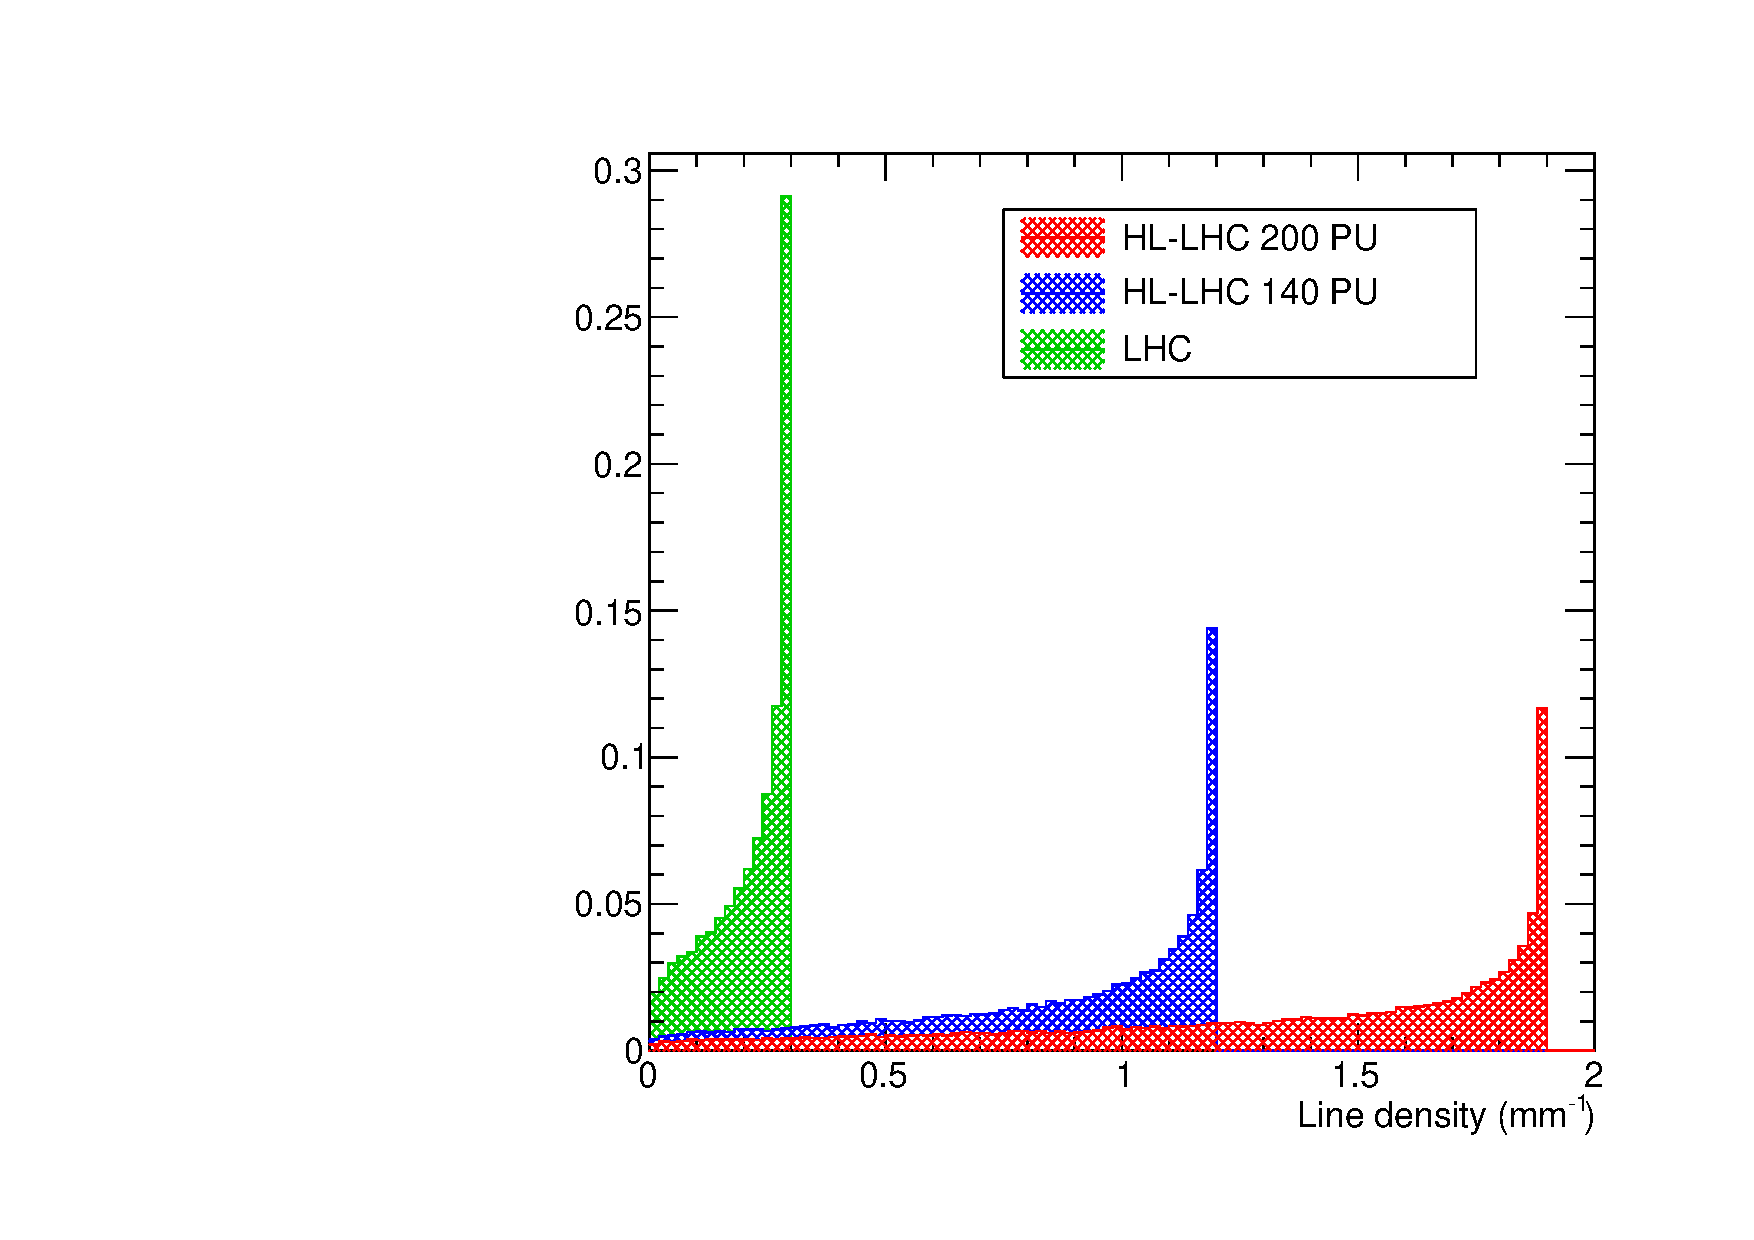
\includegraphics[width=0.325\textwidth]{figs/cms/mtd_line_density.pdf}
    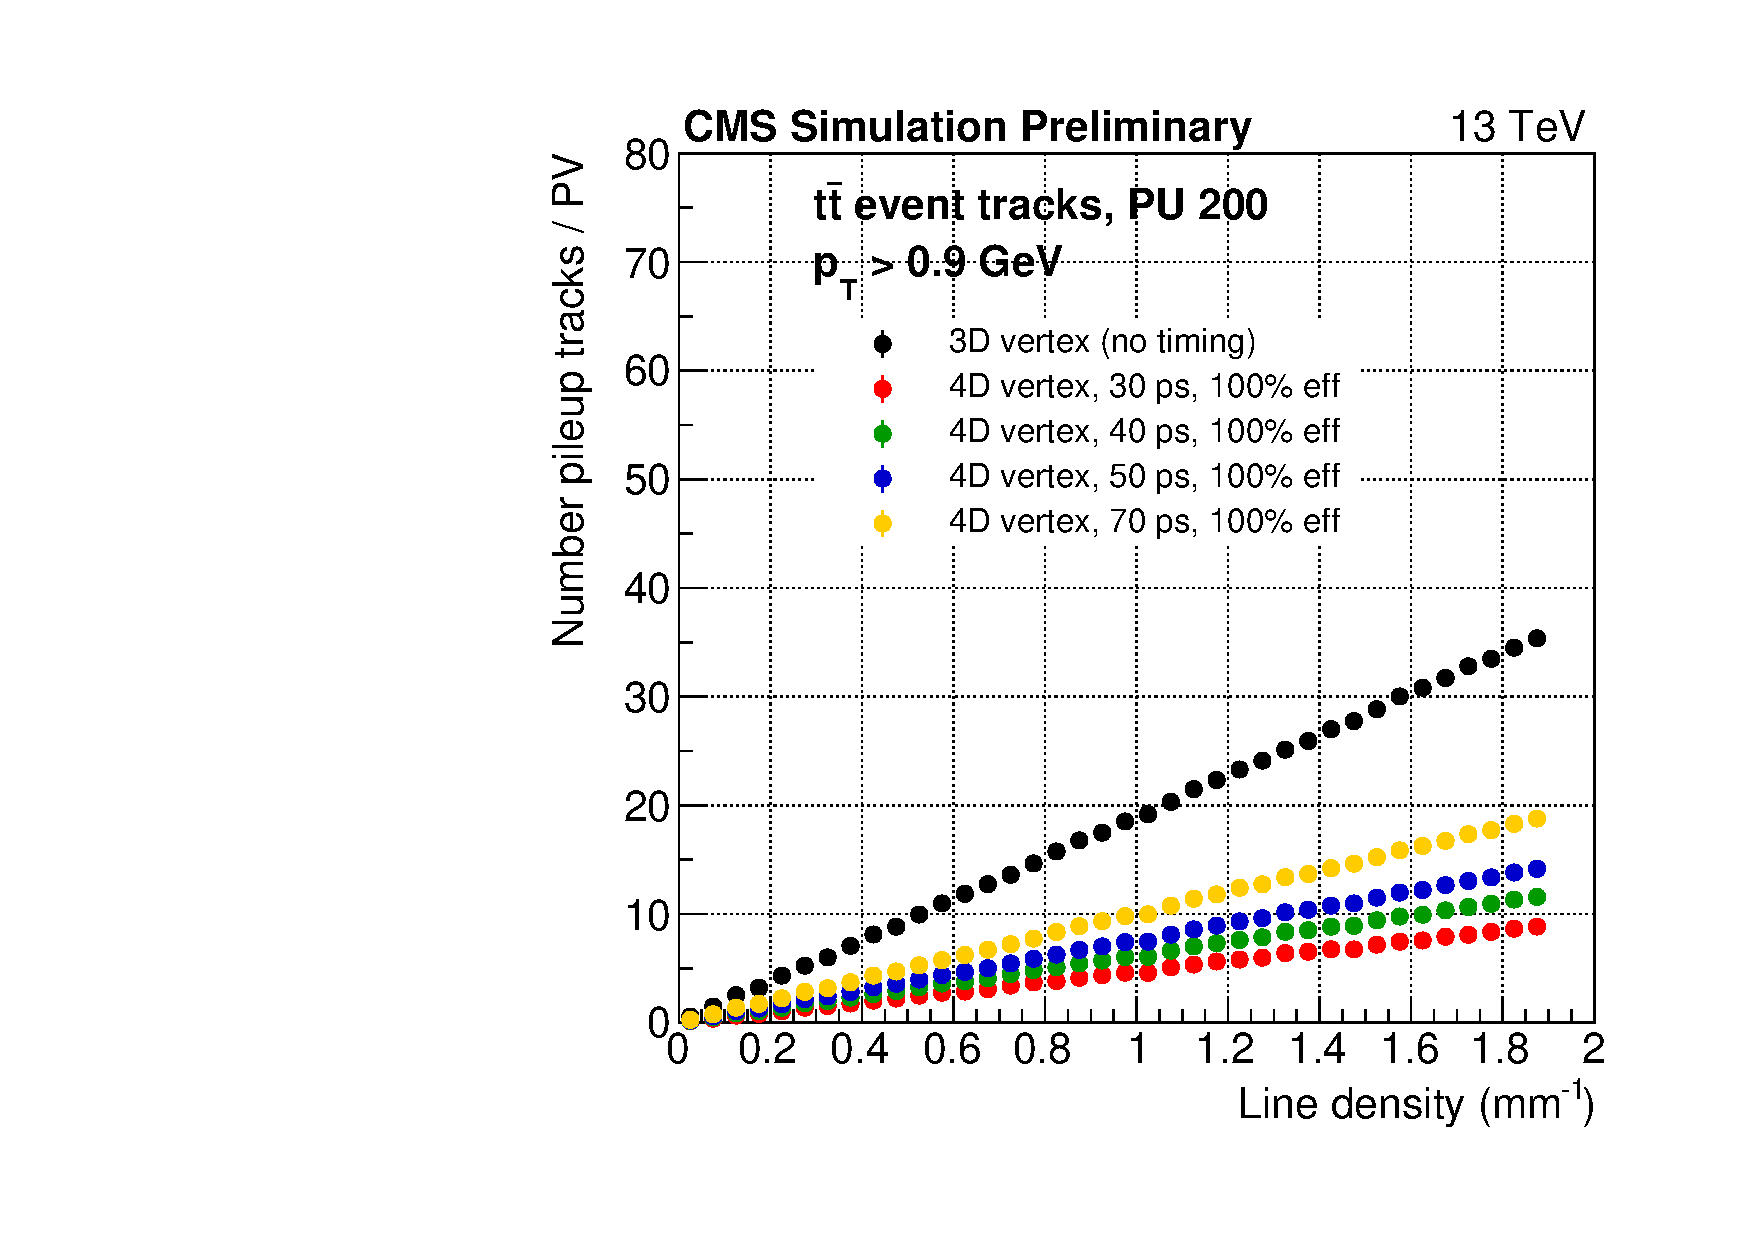
\includegraphics[width=0.325\textwidth]{figs/cms/mtd_npu_reduction.pdf}
    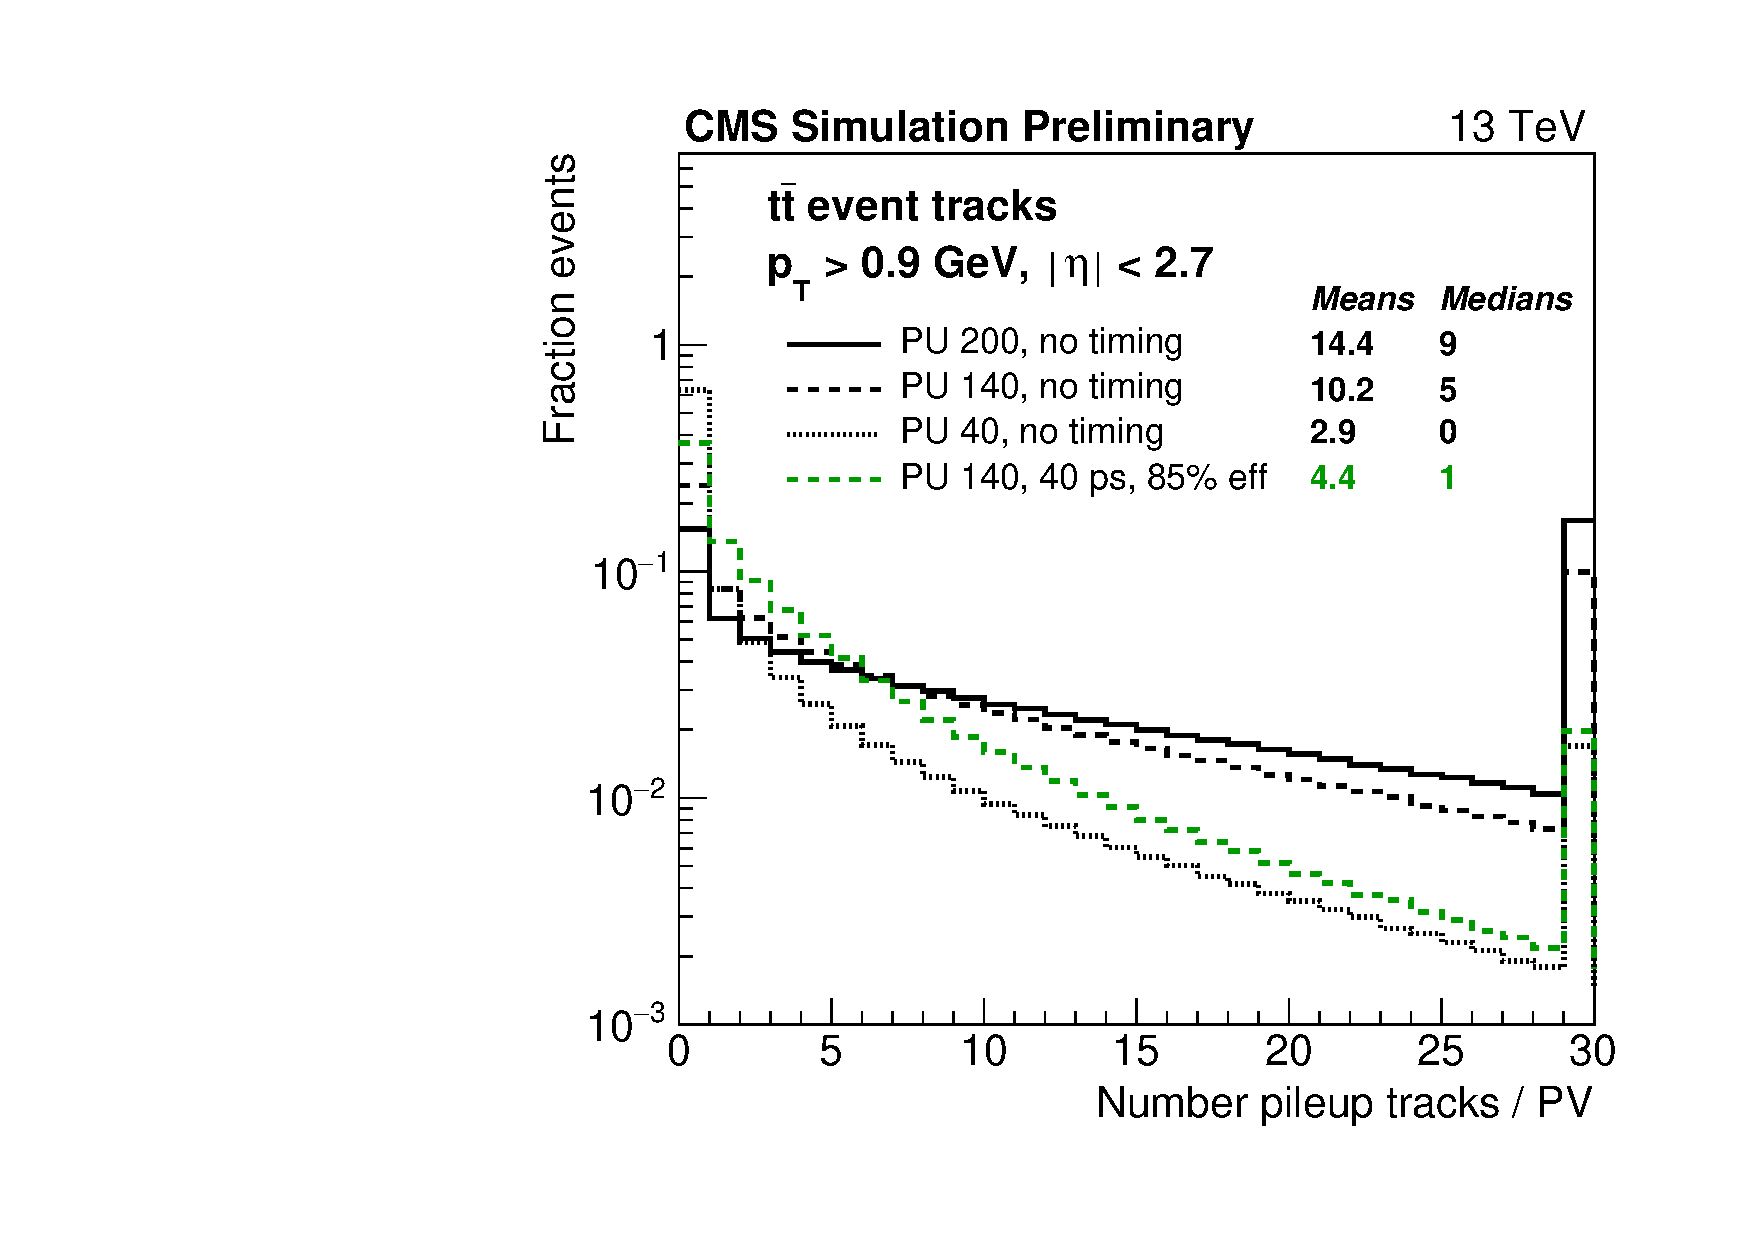
\includegraphics[width=0.325\textwidth]{figs/cms/mtd_pudist.pdf}
    \caption{(left) Distribution of line density of PU vertices for different $\langle N_\mrm{PU}\rangle$ scenarios.
      The right edges of the distributions correspond to a vertex in the center of the gaussian spatial spread
      of vertices. (middle) The mean number of PU tracks associated to the primary vertex as a function of line density,
      with no timing information and with 30, 40, 50, and 70 ps timing resolutions, assuming $\langle N_\mrm{PU}\rangle=200$.
      A resolution of $\sim$30 ps reduces the PU contamination to near present-LHC levels. (right) Distributions
      of the number of PU tracks associated to the primary vertex, assuming no timing and $\langle N_\mrm{PU}\rangle$ of
      40, 140, and 200, and under a realistic HL-LHC scenario of $\langle N_\mrm{PU}\rangle=140$ with a timing layer
      with $\sigma_{t}=40$ ps and an efficiency of 85\%.
            }
    \label{fig:mtd_pured}
  \end{center}
\end{figure}

The idea is to add a ``fourth dimension'' in the tracking of particles, which will allow discrimination between
spatially overlapping vertices. Pileup interactions have not only a spatial spread with and RMS of around 4.3~cm,
but also a spread in time with an RMS of 180--200~ps. An ability to measure the time of tracks with a resolution of
around 40~ps would allow an effective reduction of HL-LHC pileup to current levels. This is illustrated in
Fig.~\ref{fig:mtd_pured}, which shows the distribution of PU vertex line density under different 
$\langle N_\mrm{PU}\rangle$ scenarios, and the number of PU tracks associated to the primary vertex
as under different timing capability assumptions.

\begin{figure}[t]
  \begin{center}
    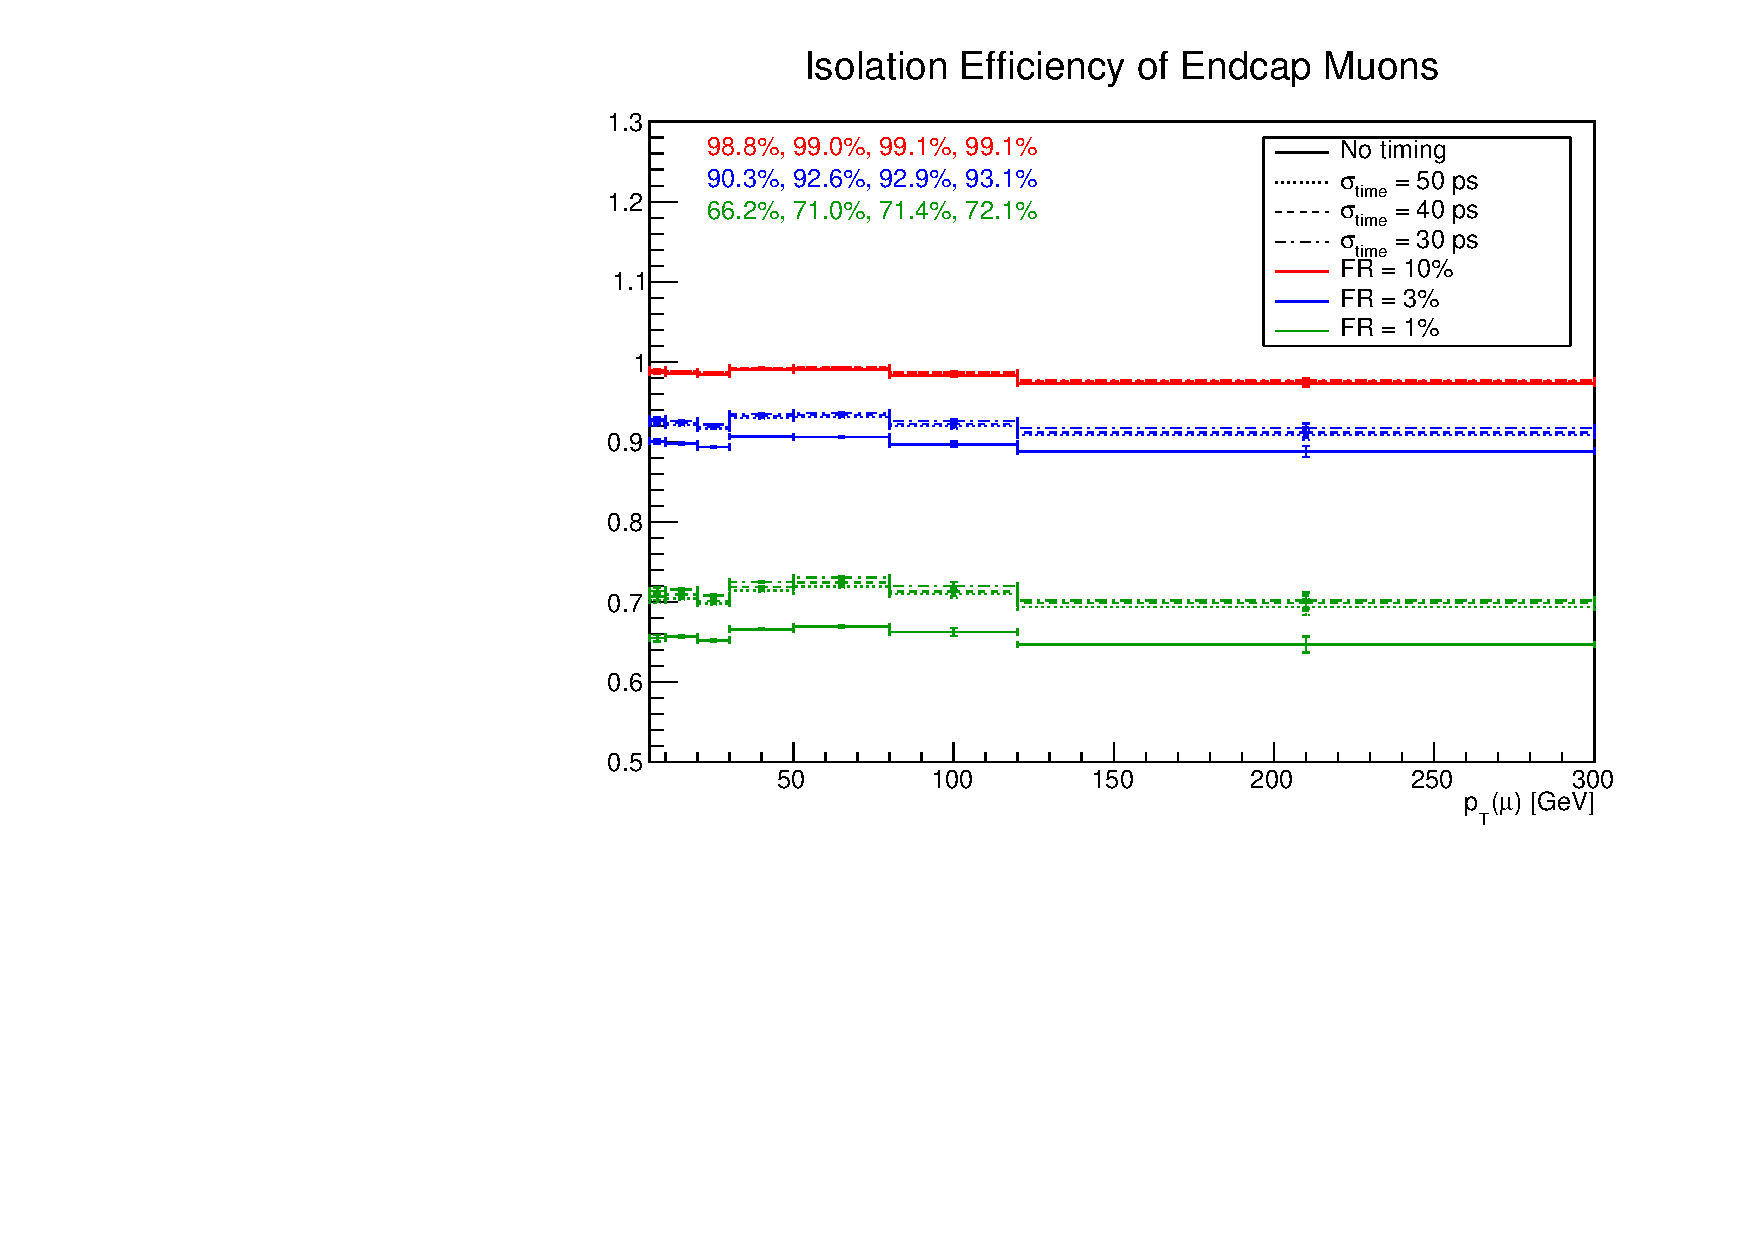
\includegraphics[width=0.49\textwidth]{figs/cms/mtd_muiso.pdf}
    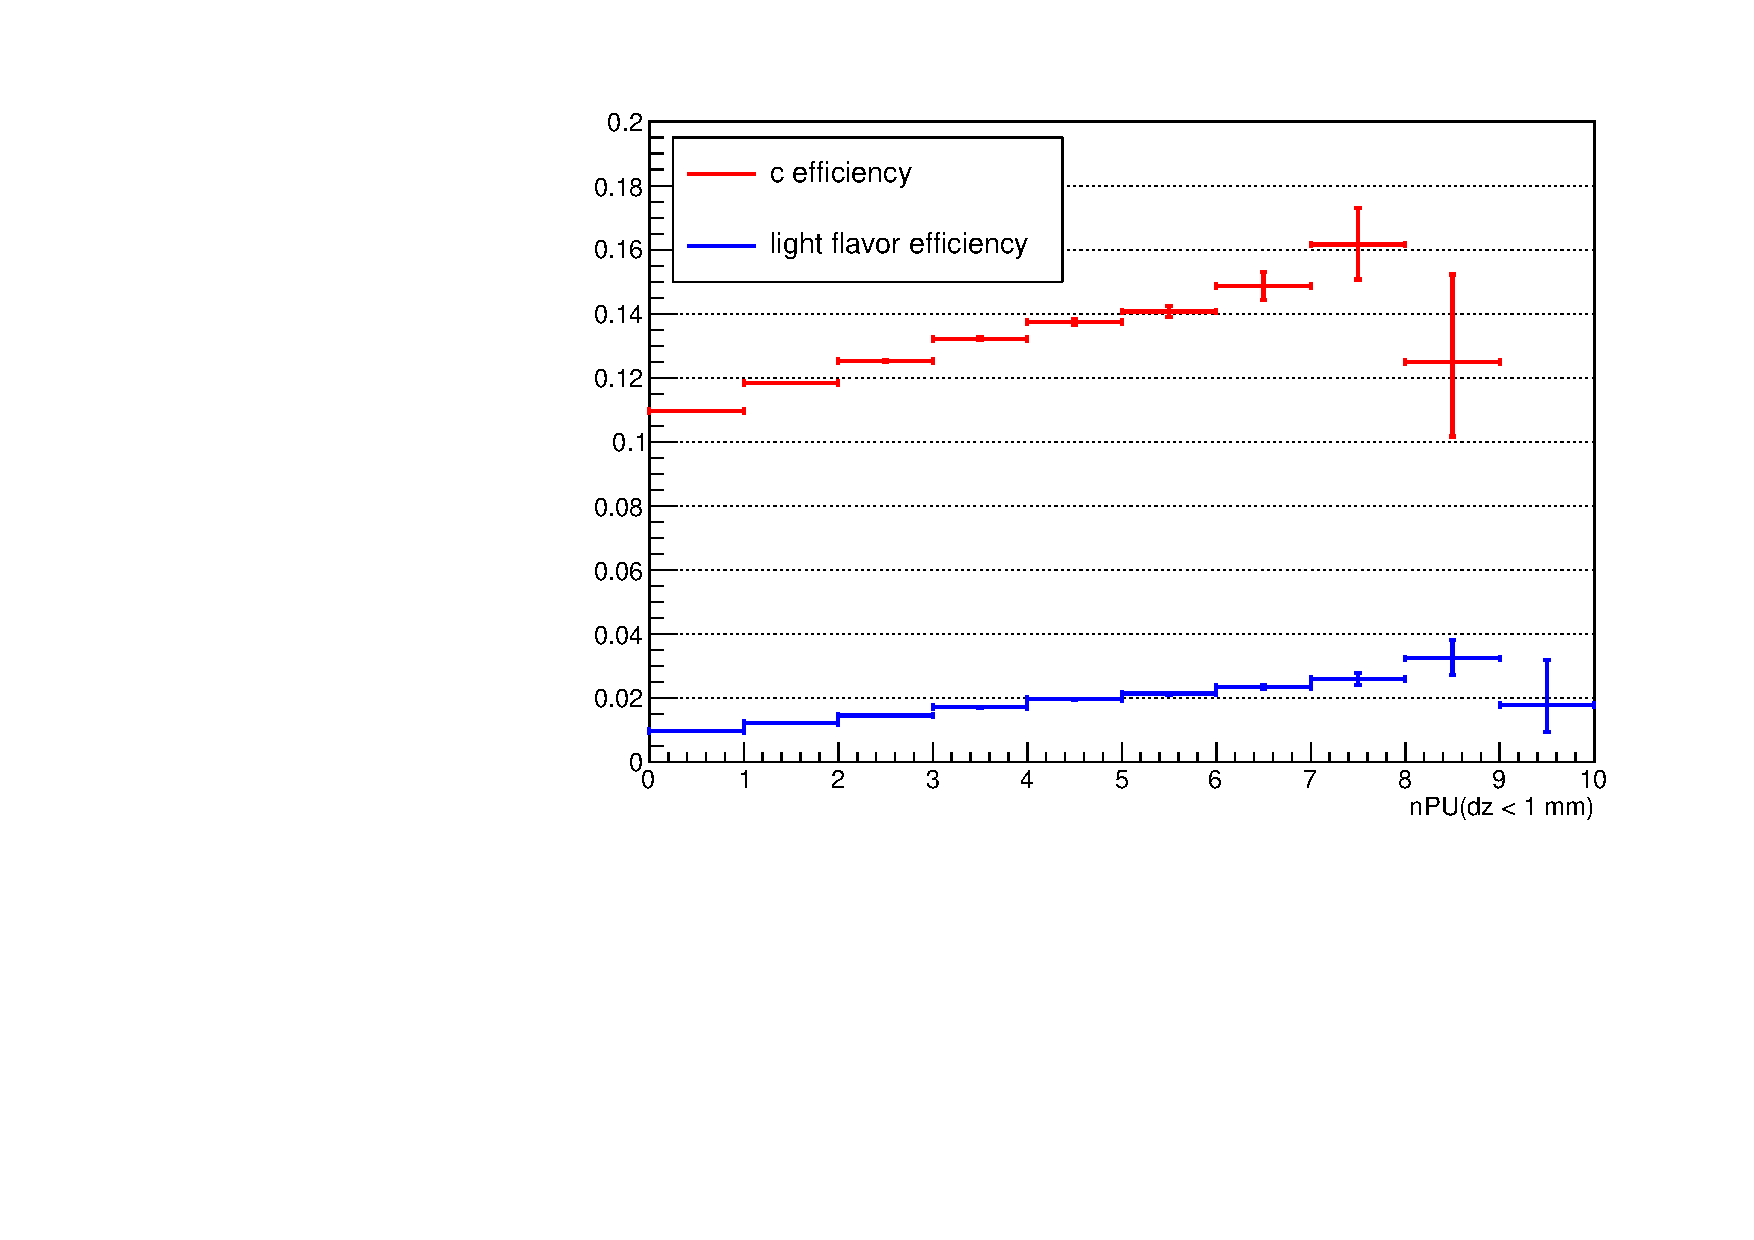
\includegraphics[width=0.49\textwidth]{figs/cms/mtd_btag.pdf}
    \caption{(left) Track isolation efficiency for prompt muons under different
      timing scenarios, for various fixed fake rates. (right) b-tagging fake rate
      for charm and light flavor quarks, as a function of the number of PU vertices
      within 1 mm of the primary vertex. Adding timing information effectively
      reduces this number.
            }
    \label{fig:mtd_isobtag}
  \end{center}
\end{figure}

In addition to reducing the raw number of PU vertices near the primary vertex, adding
timing information has visible effects on more tangible detector performance metrics
such as prompt lepton identification and b-tagging, as shown in  Fig.~\ref{fig:mtd_isobtag}.
These figures were made using generator-level tracks from \ttbar simulation, overlaying
200 random minimum-bias interaction vertices, and emulating a timing layer by smearing
each track's time by the desired resolution.

The design of the timing layer is separated into barrel and endcap components, due to
their different physics requirements. The barrel timing layer, situated between
the tracker and the ECAL, will consist
of arrays of scintillating Lutetium Yttrium Orthosilicate crystals, read out by silicon
photomultipliers. Charged particles passing through generate optical photons, which are
measured to give a timestamp of the passing particle.

The endcap detectors are closer to the beamline and hence receive much larger radiation
doses. This would degrade the performance of scintillating crystals too quickly, so silicon
low-gain avalanche detectors (LGADs)~\cite{Moffat:lgad} are used instead, which add a thin p-type multiplication layer to
traditional silicon sensors, and can achieve time resolutions of up to 20 ps.
Rows of LGAD sensors will be mounted on either side of two support disks, as shown in Fig.~\ref{fig:mtd_etl}.
Gaps are left between the rows to allow for power and cooling service channels, 
but the rows on either side of the disks are offset to provide full coverage.
The disks are mounted on the inside of the calorimeter endcap structure.

\begin{figure}[t]
  \begin{center}
    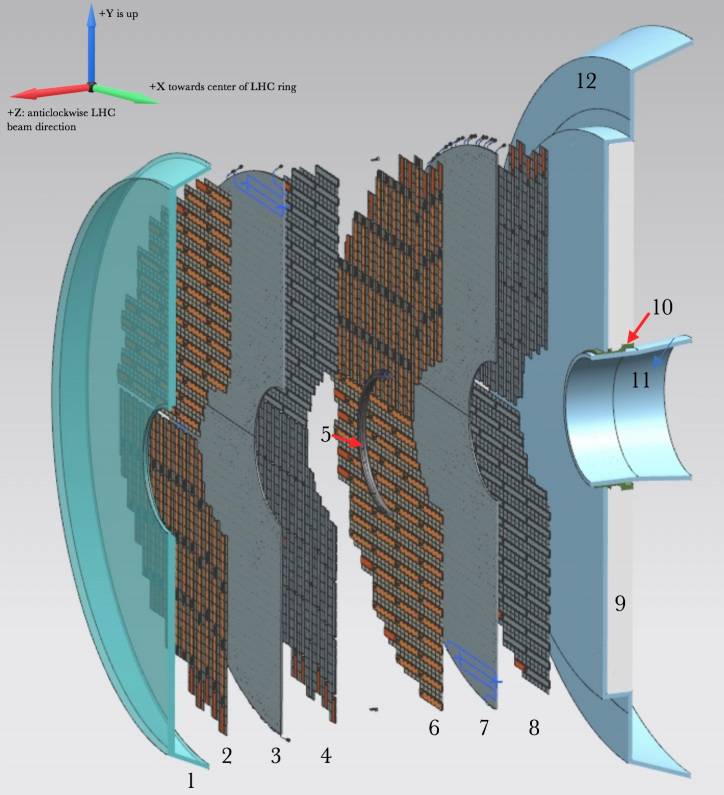
\includegraphics[width=0.49\textwidth]{figs/cms/etl.png}
    \caption{Layout of the proposed endcap timing layer. Rows of LGAD sensors
      are mounted on either side of two support disks, with the rows on either side
      offset such that full coverage is attained. (Image from~\cite{CMS:mtd})
            }
    \label{fig:mtd_etl}
  \end{center}
\end{figure}
